\documentclass{article}

%%%%%%%%%%%%%%%%%%%%%%%%%
% Packages & Macros
%%%%%%%%%%%%%%%%%%%%%%%%%

% For including graphics
\usepackage{graphicx}

% For title page
\usepackage{datetime}
\newdateformat{monthyeardate}{\monthname[\THEMONTH] \THEYEAR}

% For supporting linking
\usepackage{hyperref}
\hypersetup{colorlinks,urlcolor=blue,linkcolor=blue,anchorcolor=blue,citecolor=blue}

% For table colouring (in command line tables)
\usepackage{colortbl}

%%%%%%%%%%%%%%%%%%%%%%%%%
% Tool-Specific Macros
%%%%%%%%%%%%%%%%%%%%%%%%%
\usepackage{xspace}

\newcommand{\args}[1] {\textit{#1}}
\newcommand{\cmd}[1] {\texttt{#1}}     % Use for command window commands, e.g., \cmd{svn up}
\newcommand{\block}[1] {\textsf{#1}}   % Use for Simulink block names, e.g., \cmd{Subsystem1}
\newcommand{\signal}[1] {\textsf{#1}}   % Use for Simulink block names, e.g., \cmd{Subsystem1}
\newcommand{\ring}[1] {\textsf{#1}} 	 % Use for files names and paths
\newcommand{\keyword}[1] {\texttt{#1}} % Use for keywords of programming languages, e.g., \keyword{while}
\newcommand{\file}[1] {\texttt{#1}} 	 % Use for files names and paths
\newcommand{\param}[1] {\textsf{#1}}   % Use for block parameter names, e.g., \param{BlockType}

% Matlab Products
\newcommand{\matlab}{\textsc{Matlab}\@\xspace}
\newcommand{\Matlab}{\textsc{Matlab}\@\xspace}
\newcommand{\Simulink}{Simulink\@\xspace}
\newcommand{\simulink}{Simulink\@\xspace}
\newcommand{\SDV}{Simulink Design Verifier\@\xspace}
\newcommand{\mpath}{\Matlab search path\@\xspace}

% Block Names (not BlockType)
\newcommand{\ds}{\block{Data Store}\@\xspace}
\newcommand{\DSM}{\block{Data Store Memory}\@\xspace}
\newcommand{\DSR}{\block{Data Store Read}\@\xspace}
\newcommand{\DSW}{\block{Data Store Write}\@\xspace}
\newcommand{\DSRW}{\block{Data Store Read/Write}\@\xspace}
\newcommand{\DSMRW}{\block{Data Store Memory/Read/Write}\@\xspace}

\newcommand{\goto}{\block{Goto}\@\xspace}
\newcommand{\from}{\block{From}\@\xspace}

\newcommand{\inport}{\block{Inport}\@\xspace}
\newcommand{\outport}{\block{Outport}\@\xspace}
\newcommand{\constant}{\block{Constant}\@\xspace}
\newcommand{\ground}{\block{Ground}\@\xspace}
\newcommand{\subsystem}{\block{Subsystem}\@\xspace}

\newcommand{\logic}{\block{Logical Operator}\@\xspace}
\newcommand{\relational}{\block{Relational Operator}\@\xspace}
\newcommand{\ifblk}{\block{If}\@\xspace}
\newcommand{\switch}{\block{Switch}\@\xspace}
\newcommand{\merge}{\block{Merge}\@\xspace}

\newcommand{\docblock}{\block{DocBlock}\@\xspace}

\newcommand{\simfunc}{\block{Simulink Function}\@\xspace}
\newcommand{\simfunccaller}{\block{Function Caller}\@\xspace}

\newcommand{\toworkspace}{\block{To Workspace}\@\xspace}
\newcommand{\fromworkspace}{\block{From Workspace}\@\xspace}

\newcommand{\tofile}{\block{To File}\@\xspace}
\newcommand{\fromfile}{\block{From File}\@\xspace}

\newcommand{\fromspreadsheet}{\block{From Spreadsheet}\@\xspace}

\newcommand{\modelref}{\block{Model Reference}\@\xspace}
\newcommand{\library}{\block{Library}\@\xspace}
\newcommand{\librarylink}{\block{Library Link}\@\xspace}

% Commonly used parameters
\newcommand{\AND}{\param{AND}\@\xspace}
\newcommand{\OR}{\param{OR}\@\xspace}
\newcommand{\NOT}{\param{NOT}\@\xspace}
\newcommand{\NOR}{\param{NOR}\@\xspace}
\newcommand{\NAND}{\param{NAND}\@\xspace}
\newcommand{\XOR}{\param{XOR}\@\xspace}
\newcommand{\NXOR}{\param{NXOR}\@\xspace}

% Common Abbreviations
% Example
\newcommand{\eg}{\textrm{e.g.,}\@\xspace}

% That Is To Say
\newcommand{\ie}{\textrm{i.e.,}\@\xspace}

% And So On
\newcommand{\etc}{\textrm{etc.}\@\xspace}

% And Others
\newcommand{\etal}{\textrm{et al.}\@\xspace}

% With Respect To
\newcommand{\wrt}{\textrm{w.r.t.}\@\xspace}

% Vice Versa
\newcommand{\vrsa}{\textrm{vice versa}\@\xspace}

% Symbols

\usepackage{amssymb}
\newcommand{\checkbox}{\makebox[0pt][l]{$\square$}\raisebox{.15ex}{\hspace{0.1em}$\checkmark$}}%
\newcommand{\uncheckbox}{$\square$~}%


\newcommand{\ToolName}{Flatten Subsystem\@\xspace}

\newcommand{\menu}[1]{%
	\ifthenelse{\equal{#1}{1}}{Flatten Subsystem}{}%
  	\ifthenelse{\equal{#1}{2}}{?}{}%
}

\newcommand{\func}[1]{%
	\ifthenelse{\equal{#1}{1}}{FlattenSybsystem}{}%
	\ifthenelse{\equal{#1}{2}}{?}{}%
	\ifthenelse{\equal{#1}{3}}{?}{}%
  	\ifthenelse{\equal{#1}{4}}{?}{}%
  	\ifthenelse{\equal{#1}{5}}{?}{}%
  	\ifthenelse{\equal{#1}{6}}{?}{}%
}

\newcommand{\toolFolder}{\cmd{FlattenSubsystem}}
\newcommand{\demoName}{\cmd{FlattenSubsystemtDemo}\@\xspace}

\newcommand{\FCA}{0} 	% Enable/disabled FCA-specific content	
\newcommand{\HowSetPath}{\ifthenelse{\equal{\FCA}{1}}{If it is not, go to \cmd{File~>~Set~Path...}, press \cmd{Add with Subfolders}, and select the \cmd{McMaster\_Tools} folder. Restart \matlab after doing so.}{}}

%%%%%%%%%%%%%%%%%%%%%%%%%
% Document
%%%%%%%%%%%%%%%%%%%%%%%%%

\title{\ToolName Tool}
\date{\monthyeardate\today}

\begin{document}

%%%%%%%%%%%%%%%%%%%%%%%%%%%%%%%%%%%%%%%%%%%%%%%%%%%%%%%%%%%%%%%%%%%
% Title Page
%%%%%%%%%%%%%%%%%%%%%%%%%%%%%%%%%%%%%%%%%%%%%%%%%%%%%%%%%%%%%%%%%%%
\maketitle
\vfill

\begin{figure}
	\centering
	
\includegraphics[]{../figs/McSCert_Logo.pdf} \\
	McMaster Centre for Software Certification (McSCert)
\end{figure}

\newpage

%%%%%%%%%%%%%%%%%%%%%%%%%%%%%%%%%%%%%%%%%%%%%%%%%%%%%%%%%%%%%%%%%%%
% Table of Contents
%%%%%%%%%%%%%%%%%%%%%%%%%%%%%%%%%%%%%%%%%%%%%%%%%%%%%%%%%%%%%%%%%%%
\tableofcontents
\newpage

%%%%%%%%%%%%%%%%%%%%%%%%%%%%%%%%%%%%%%%%%%%%%%%%%%%%%%%%%%%%%%%%%%%
% Introduction
%%%%%%%%%%%%%%%%%%%%%%%%%%%%%%%%%%%%%%%%%%%%%%%%%%%%%%%%%%%%%%%%%%%
\section{Introduction}

% Briefly, what is the tool?
The \ToolName tool automatically flattens a Simulink subsystem, that is, it moves the subsystem contents up one level, reconnects the signals, and removes the subsystem block. This tool is useful for making quick transformations to a model by automating the tedious task of manually copying and connecting the many elements contained in a subsystem.

\textit{Note: This functionality has been since included in \matlab/Simulink 2014a as the ``Expand Subsystem" operation\footnote{\url{https://www.mathworks.com/help/simulink/ug/expand-subsystem-contents.html}}. This tool is still beneficial for earlier versions of \matlab/Simulink, as well as handling more types of subsystems}

% Is there more information?
\subsection{More Information}
For more information on the tool and how it can be used in a model-based development with Simulink, please refer to the following papers:

\vspace{1em}
Vera Pantelic, Steven Postma, Mark Lawford, Monika Jaskolka, Bennett Mackenzie, Alexandre Korobkine, Marc Bender, Jeff Ong, Gordon Marks, Alan Wassyng, \href{https://link.springer.com/article/10.1007/s10009-017-0450-9}{``Software engineering practices and Simulink: bridging the gap,"} \textit{International Journal on Software Tools for Technology Transfer (STTT)}, 2017, 95--117.

\vspace{1em}
Vera Pantelic, Steven Postma, Mark Lawford, Alexandre Korobkine, Bennett Mackenzie, Jeff Ong, and Marc Bender, \href{http://www.cas.mcmaster.ca/~lawford/papers/MODELSWARD2015.pdf}{``A Toolset for Simulink: Improving Software Engineering Practices in Development with Simulink,"}\textit{Proceedings of 3rd International Conference on Model-Driven Engineering and Software Development (MODELSWARD 2015)}, SCITEPRESS, 2015, 50--61.

\newpage	
%%%%%%%%%%%%%%%%%%%%%%%%%%%%%%%%%%%%%%%%%%%%%%%%%%%%%%%%%%%%%%%%%%%
% How to Use the Tool
%%%%%%%%%%%%%%%%%%%%%%%%%%%%%%%%%%%%%%%%%%%%%%%%%%%%%%%%%%%%%%%%%%%
\section{How to Use the Tool}
This section describes what must be done to setup the tool, as well as how to use the tool.

%---------------------------------------
% What needs to be done before the tool can be used? 
% What needs to be done to a model in order for it to work on said model?
%---------------------------------------
\subsection{Prerequisites and Installation}

\begin{enumerate}
	\item Use \Matlab/\Simulink 2011b or newer.
	\item Install the \href{https://github.com/McSCert/Auto-Layout}{Auto Layout Tool}.
	\item To install the tool,
	\begin{enumerate}
		\item from a \file{.zip} file --- unzip the contents into your desired location. Ensure the unzipped folder and subfolders are present in your \mpath, or add them if they are not present. Run \href{https://www.mathworks.com/help/simulink/ug/registering-customizations.html}{sl\_refresh\_customizations} to refresh the Context Menu. 
		\item from a \file{.mltbx} file --- simply open \Matlab and double-click on the file. Your \mpath should be automatically configured.
		\item from the files only --- add the folders and subfolders to your \mpath. Run \href{https://www.mathworks.com/help/simulink/ug/registering-customizations.html}{sl\_refresh\_customizations} to refresh the Context Menu.
	\end{enumerate}
	\begin{itemize}
		\item \textit{Note:} If running the command ``\cmd{which FlattenSubsystem}'' indicates that the script is not found, then the tool needs to be added to the \mpath.
		For information on adding files to the \mpath, please see the \href{https://www.mathworks.com/help/matlab/matlab_env/add-remove-or-reorder-folders-on-the-search-path.html}{MathWorks documentation}.
	\end{itemize}
	\item Ensure the Simulink-Utility folder is on your \mpath. This is a dependency for the tool to work correctly.
	\item Ensure your model is open (or loaded, for command line use) and unlocked.
\end{enumerate}

%---------------------------------------
% How/when do you access the tool?
%---------------------------------------
\subsection{Getting Started}
The tool can be used via the Simulink Context Menu, which can be viewed by right-clicking in a model. The \emph{\menu{1}} option is available, as shown in Figure~\ref{FIG:contextMenu}.

\begin{figure}[!ht]
	\centering
	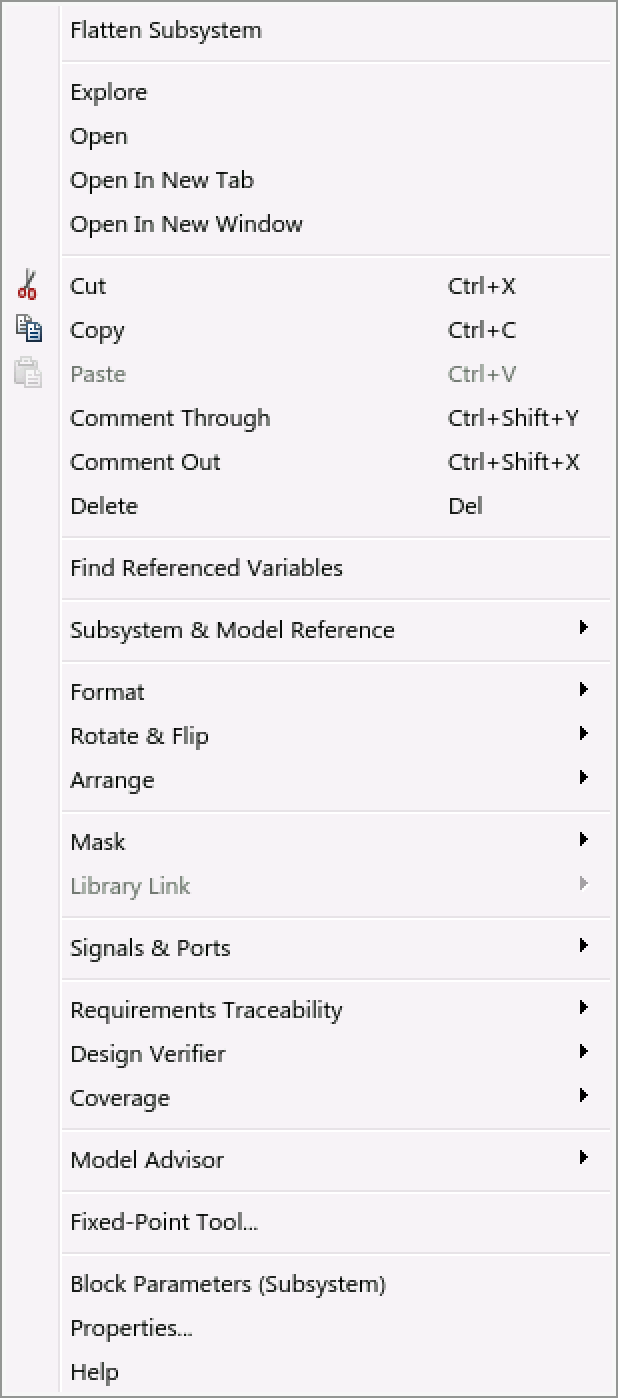
\includegraphics[width=0.5\textwidth]{../figs/ContextMenu}
	\caption{Simulink Context Menu with tool option visible.}
	\label{FIG:contextMenu}
\end{figure}

%---------------------------------------
% What are the main uses of the tool?
%---------------------------------------
\subsection{Functionality}

%This section describes the tool functionality when being used from the Simulink Context Menu.

Right-clicking on a subsystem in the model and then selecting \cmd{\menu{1}} from the Context Menu will flatten those subsystems. Any blocks that are considered subsystems can be flattened, including atomic subsystems, code reused subsystems, etc. These types of subsystems are not supported with Simulink's built-in \cmd{Expand Subsystem} function.

%{\color{red} 
%\begin{itemize}
%	\item Atomic subsystems
%	\item Conditional subsystems
%	\item Configurable subsystems
%	\item Variant subsystems
%	\item Subsystems in a referenced model
%	\item Subsystems with the Read/Write permissions parameter set to ReadOnly or NoReadWrite
%	\item Subsystems with an InitFcn, StartFcn, PauseFcn, ContinueFcn, or StopFcn callback
%	\item Subsystems with linked requirements (using Simulink Verification and Validation software)
%\end{itemize}
%}
%---------------------------------------
% What else does the tool do?
%---------------------------------------
\subsection{Errors and Warnings}
Any errors or warnings during tool use will be visible in the \matlab Command Window. Typically, errors will be shown when the model is locked or function parameters are incorrect.


%%%%%%%%%%%%%%%%%%%%%%%%%%%%%%%%%%%%%%%%%%%%%%%%%%%%%%%%%%%%%%%%%%%
% Example
%%%%%%%%%%%%%%%%%%%%%%%%%%%%%%%%%%%%%%%%%%%%%%%%%%%%%%%%%%%%%%%%%%%
\section{Example}

Use the command \demoName in the Simulink command window to open the example model, shown in Figure~\ref{FIG:demo1} and~\ref{FIG:demo2}. This simple example has a single subsystem, which contains a few blocks. 

\begin{figure}[ht!]
	\centering
	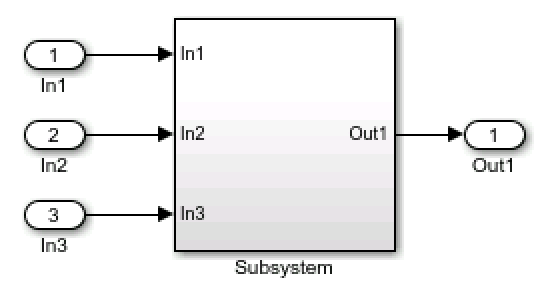
\includegraphics[scale=.55]{../figs/Demo1}
	\caption{\ToolName demo: The \demoName model before flattening the subsystem.}
	\label{FIG:demo1}
\end{figure}

\begin{figure}[ht!]
	\centering
	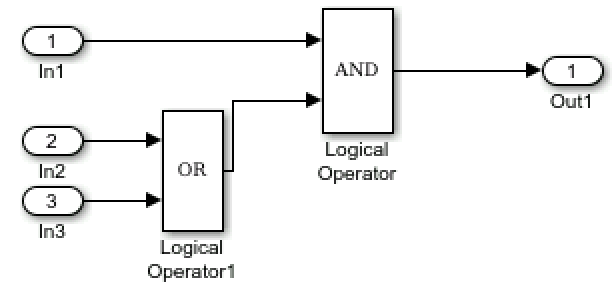
\includegraphics[scale=.55]{../figs/Demo2}
	\caption{\ToolName demo: The subsystem from Figure~\ref{FIG:demo1} before flattening.}
	\label{FIG:demo2}
\end{figure}

To flatten this subsystem, right-click on the subsystem in Figure~\ref{FIG:demo1} and select the \cmd{\menu{1}} option. The resulting model is shown in Figure~\ref{FIG:demo3}. 

\begin{figure}[ht!]
	\centering
	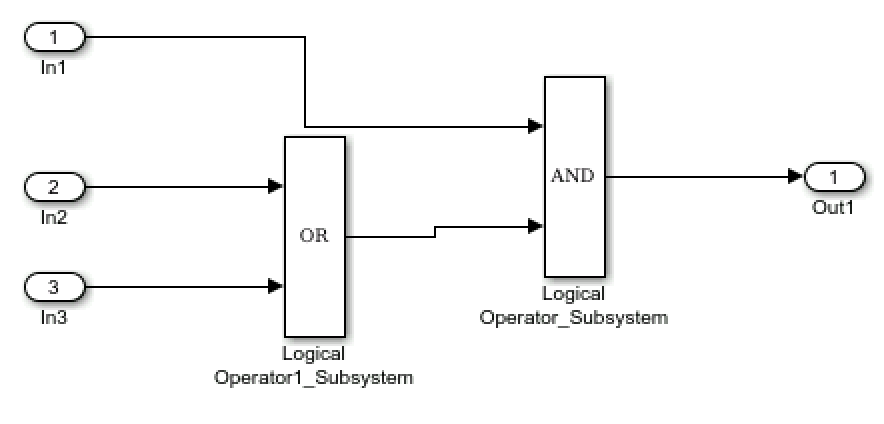
\includegraphics[scale=.55]{../figs/Demo3}
	\caption{\ToolName demo: The \demoName model after flattening.}
	\label{FIG:demo3}
\end{figure}

%%%%%%%%%%%%%%%%%%%%%%%%%%%%%%%%%%%%%%%%%%%%%%%%%%%%%%%%%%%%%%%%%%%
% Matlab Commands
%%%%%%%%%%%%%%%%%%%%%%%%%%%%%%%%%%%%%%%%%%%%%%%%%%%%%%%%%%%%%%%%%%%
\clearpage
\section{Matlab Commands}

The tool can also be used via the \matlab command line, with the following function.

%%---------------------------------------
%% Command 1
%%---------------------------------------
\begin{center}
	\begin{tabular}{| >{\columncolor[gray]{0.9}}l | p{10.5cm} |} \hline
		Function 		& \cmd{\func{1}} \\ \hline
		Syntax			& \cmd{\func{1}}(\args{address}, \args{subToFlatten}) \\ \hline
		Description		& Takes all blocks in \args{subToFlatten} and moves them to up one level, while also removing the subsystem. \\ \hline
		Inputs			& \args{address}: Simulink model name. \\ 
								& \args{subToFlatten}: Cell array of subsystems to flatten. \\ \hline
		Outputs			& N/A\\ \hline	
	\end{tabular}
\end{center}

%{\color{red}MB: Does the tool actually create a new model and replace the old one? GM: The tool just edits the model to my knowledge (in theory the old stuff could do something funny with creating a new model, but I'm fairly sure it doesn't).}



%%%%%%%%%%%%%%%%%%%%%%%%%%%%%%%%%%%%%%%%%%%%%%%%%%%%%%%%%%%%%%%%%%%
% Example
%%%%%%%%%%%%%%%%%%%%%%%%%%%%%%%%%%%%%%%%%%%%%%%%%%%%%%%%%%%%%%%%%%%

%\vspace{2em}
%
%\paragraph{Example:} The following commands perform the same operations as described previously for the \demoName example, however via the Matlab command line.
%
%\begin{enumerate}
%	\item \cmd{open\_system(`\demoName')}	
%	\item \cmd{\func{2}(`\demoName', 0, 0, `All', 0)}
%	\item \cmd{\func{1}(`\demoName', 1, 1, `All', 0)} 										
%	\item \cmd{\func{3}(`\demoName')}								
%\end{enumerate}

\end{document}